% VUT FIT MITAI
% MSZ 2021/2022
% Author: Vladimir Dusek
% Login: xdusek27

%%%%%%%%%%%%%%%%%%%%%%%%%%%%%%%%%%%%%%%%%%%%%%%%%%%%%%%%%%%%%%%%%%%%%%%%%%%%%%%%

% Path to figures
\graphicspath{{msp/randomizovane_algoritmy/figures}}

%%%%%%%%%%%%%%%%%%%%%%%%%%%%%%%%%%%%%%%%%%%%%%%%%%%%%%%%%%%%%%%%%%%%%%%%%%%%%%%%

\chapter{MSP~--~Randomizované algoritmy (Monte Carlo a Las Vegas algoritmy).}

%%%%%%%%%%%%%%%%%%%%%%%%%%%%%%%%%%%%%%%%%%%%%%%%%%%%%%%%%%%%%%%%%%%%%%%%%%%%%%%%

\section{Zdroje}

\begin{compactitem}
    \item \path{MSP_13_Randomized_Algorithms.pdf}
    \item \path{MSP_2021-12-14_1080p.mp4}
\end{compactitem}

%%%%%%%%%%%%%%%%%%%%%%%%%%%%%%%%%%%%%%%%%%%%%%%%%%%%%%%%%%%%%%%%%%%%%%%%%%%%%%%%

\section{Úvod a kontext}

\begin{compactitem}
    \item K čemu jsou randomizované algoritmy? \begin{compactitem}
        \item Analyzujeme průměrné chování algoritmů (nikoliv nejhorší případ).

        \item Randomizací také můžeme dosáhnout snížení očekávané ceny algoritmu.
    \end{compactitem}

    \item Přesahuje rámec analýzy nejlepšího nebo nejhoršího případu. \begin{compactitem}
        \item Analýza všech případů (vstupů) pomocí jejich pravděpodobnostního rozdělení.

        \item V mnoha případech poskytuje lepší vhled do praktické složitosti.

    \end{compactitem}

    \item Existují dva přístupy k randomizaci: \begin{compactitem}
        \item randomizace pořadí vstupů (např. Hiring Problem),

        \item randomizace volby provedené v rámci algoritmu (např. Quicksort).
    \end{compactitem}
\end{compactitem}

%%%%%%%%%%%%%%%%%%%%%%%%%%%%%%%%%%%%%%%%%%%%%%%%%%%%%%%%%%%%%%%%%%%%%%%%%%%%%%%%

\section{Hiring Problem}

\begin{compactitem}
    \item Firma chce nabrat nejlepšího zaměstnance.

    \item Můžeme randomizovat seznam kandidátů.

    \item Složitost: \begin{compactitem}
        \item nejhorší případ: $\mathcal{O}(n \cdot c_h)$
        \item nejlepší případ: $\mathcal{O}(c_h)$
    \end{compactitem}
\end{compactitem}

\begin{figure}[H]
    \centering
    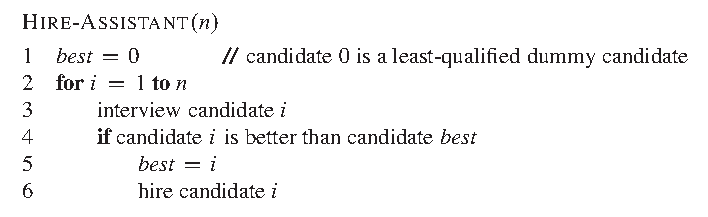
\includegraphics[width=0.8\linewidth]{hiring_problem.pdf}
    \caption{Hiring Problem v pseudokódu.}
\end{figure}

\begin{figure}[H]
    \centering
    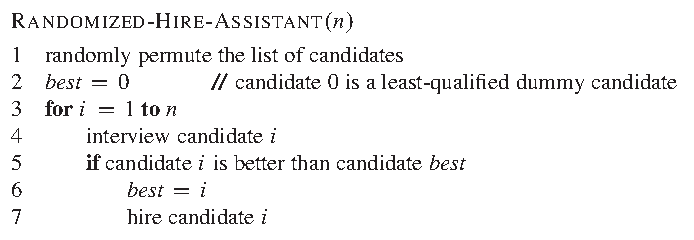
\includegraphics[width=0.8\linewidth]{hiring_problem_randomized.pdf}
    \caption{Hiring Problem randomizovaný v pseudokódu.}
\end{figure}

%%%%%%%%%%%%%%%%%%%%%%%%%%%%%%%%%%%%%%%%%%%%%%%%%%%%%%%%%%%%%%%%%%%%%%%%%%%%%%%%

\section{Indikátorová náhodná proměnná (\textit{indicator random variable})}

\begin{compactitem}
    \item Mějme prostor jevů $S$ a událost $A \in S$.

    \item Indikátorová náhodná proměnná pro $A$:
    $$ I\{A\} = \left\{
        \begin{array}{ll}
            1 & \text{pokud A nastane} \\
            0 & \text{jinak}
        \end{array}
    \right. $$

    \item Nechť $X_A = I\{A\}$, pak platí, že $E[X_A] = Pr\{A\}$ (pravděpodobnost události A).

    \item Hlavní myšlenka: Vyjádřit očekávání náhodné proměnné ($X$) jako očekávání sum komponent, které se snáze počítají (indikátorové proměnné $X_i$).

\end{compactitem}

\paragraph*{Příklad 1} Jaký je očekávaný počet padnutí orla při $n$ hodů mincí?
$$ X_i = I\{ \text{i-tý hod mincí, kdy padne orel} \}$$
$$ X = \sum_{i=1}^n X_i$$
$$ E[X] = E \left[ \sum_{i=1}^n X_i \right] = \frac{n}{2}$$

\paragraph*{Příklad 2} Jaký je očekávaný počet nalezení nejlepšího kandidáta v Hiring Problem? \begin{compactitem}
    \item Indikátorová proměnná.
    $$ X_i = I\{ \text{i-tý kandidát je přijat} \}$$

    \item Celkový počet přijatých kandidátů (cena).
    $$ X = \sum_{i=1}^n X_i$$

    \item Očekávaná cena algoritmu.
    $$ E[X] $$

    \item Pravděpodobnost, že i-tý kandidát je přijat (kandidát i je přijat, pokud je lepší, než všichni předchozí).
    $$ E[X_i] = \frac{1}{i}$$
    $$ E[X] = E \left[ \sum_{i=1}^n X_i \right] = \sum_{i=1}^n E \left[ X_i \right] = \sum_{i=1}^n \frac{1}{i} = \ln{n} + \mathcal{O}(1)$$

    \item Pravděpodobnostní analýza nám dává asymptotický lepší ohraničení ceny

    $$ \mathcal{O}(\log{n} \cdot c_h) ~~~\text{vs}~~~ \mathcal{O}(n \cdot c_h)$$

\end{compactitem}

%%%%%%%%%%%%%%%%%%%%%%%%%%%%%%%%%%%%%%%%%%%%%%%%%%%%%%%%%%%%%%%%%%%%%%%%%%%%%%%%

\section{Las Vegas}

\begin{compactitem}
    \item Pro každý vstup dává správné výsledky (korektnost je zaručena).

    \item Pro každý vstup existuje pravděpodobnost, že doba běhu bude větší než je žádoucí / očekávané.

    \item Todo: čas běhu je náhodná proměnná
\end{compactitem}

\paragraph*{Příklad X} Je dáno pole $A[1, 2, \dots, n]$ s $n$ prvky (kde $n$ je sudé). Polovina z prvků obsahuje nuly, druhá polovina obsahuje jedničky. Cíl: Najděte index který obsahuje jedničku. Zkonstruujte Las Vegas algoritmus.

\bigskip\noindent\begin{minipage}{\linewidth}
\begin{lstlisting}[language=Python, caption={Las Vegas}]
def las_vegas(A, n):
    while True:
        i = random_int(0, n)
        if A[i] == 1:
            return i
\end{lstlisting}
\end{minipage}

\begin{compactitem}
    \item Složitost $\mathcal{O}(1)$.
    \item Důkaz očekávané doby běhu s využitím indikátorové proměnné:
    $$ X_i = \left\{
        \begin{array}{ll}
            1 & \text{pokud algoritmus provede i-té porovnání} \\
            0 & \text{jinak}
        \end{array}
    \right. $$
    $$ X = \sum_{i=1}^{\infty} X_i $$
    $$ E[X] = E \left[ \sum_{i=1}^{\infty} X_i \right] = \sum_{i=1}^{\infty} E \left[ X_i \right] = \sum_{i=1}^{\infty} Pr\{ X_i \} =\sum_{i=1}^{\infty} \left(\frac{1}{2}\right)^{i-1} = 2$$
\end{compactitem}

%%%%%%%%%%%%%%%%%%%%%%%%%%%%%%%%%%%%%%%%%%%%%%%%%%%%%%%%%%%%%%%%%%%%%%%%%%%%%%%%

\section{Monte Carlo}

\begin{compactitem}
    \item Pro každý vstup existuje pravděpodobnost výskytu chyby (nesprávného výsledku).

    \item Je zaručena doba běhu algoritmu.

    \item Využívá tzv. aplicikaci.

    \item todo: Quicksort -- randomizace výběru pivota
\end{compactitem}

\paragraph*{Příklad X} Je dáno pole $A[1, 2, \dots, n]$ s $n$ prvky (kde $n$ je sudé). Polovina z prvků obsahuje nuly, druhá polovina obsahuje jedničky. Cíl: Najděte index který obsahuje jedničku. Zkonstruujte Monte Carlo algoritmus.

\bigskip\noindent\begin{minipage}{\linewidth}
\begin{lstlisting}[language=Python, caption={Monte Carlo}]
def monte_carlo(A, n):
    limit = 1000
    for _ in range(0, limit):
        i = random_int(0, n)
        if A[i] == 1:
            return i
    return None
\end{lstlisting}
\end{minipage}

\begin{compactitem}
    \item Složitost $\mathcal{O}(1)$.
\end{compactitem}
